\documentclass[conference]{IEEEtran}
\usepackage[utf8]{inputenc}
\usepackage[T1]{fontenc}
\usepackage[spanish,es-nodecimaldot]{babel}
\usepackage{amsmath,amssymb}
\usepackage{graphicx}
\usepackage{booktabs}
\usepackage{siunitx}
\usepackage{cite}
\usepackage{url}
\usepackage{float}
\graphicspath{{figures/}}

\title{Determinación experimental de la aceleración gravitatoria mediante análisis de video}
\author{\IEEEauthorblockN{Nombre del estudiante}
\IEEEauthorblockA{Curso o laboratorio\\Institución\\Correo electrónico}}

\begin{document}
\maketitle
% Archivo generado automáticamente por src/main.py; no editar manualmente.
\newcommand{\MeasuredAcceleration}{9.7863}
\newcommand{\AccelerationUncertainty}{0.0321}
\newcommand{\FitRSquared}{0.99999}
\newcommand{\FitRMSE}{0.00294}
\newcommand{\GravityRelativeError}{0.241}
\newcommand{\ValidDataPoints}{51}
\newcommand{\DroppedDataPoints}{0}


\begin{abstract}
Se presenta un flujo reproducible para analizar un experimento demostrativo de caída libre a partir de coordenadas extraídas de video. Los datos incluidos con el repositorio son sintéticos y sirven únicamente para verificar el software. La posición se registra mediante Tracker, se inspecciona en QtiPlot y se procesa con Python. Un ajuste cuadrático permite estimar la aceleración vertical, cuantificar incertidumbres y contrastar el resultado con la magnitud de referencia de la gravedad. Los valores numéricos y figuras se incorporan desde archivos generados automáticamente por el pipeline.
\end{abstract}

\begin{IEEEkeywords}
caída libre, Tracker, análisis de video, cinemática, regresión no lineal, incertidumbre
\end{IEEEkeywords}

\section{Introducción}
La caída libre es un modelo de movimiento con aceleración aproximadamente constante cuando la resistencia del aire es despreciable. El análisis de video permite obtener la posición de un objeto en función del tiempo y estimar la aceleración a partir de un ajuste de segundo grado. El objetivo es documentar un procedimiento trazable desde el dato crudo hasta el resultado estadístico.

\section{Fundamento teórico}
Para un eje vertical $y$ y aceleración constante,
\begin{equation}
 y(t)=y_0+v_0t+\frac{1}{2}a_yt^2.
 \label{eq:position}
\end{equation}
La velocidad y aceleración son $v_y(t)=v_0+a_yt$ y $a_y(t)=a_y$. El signo de $a_y$ depende de la orientación del eje vertical en Tracker; por ello, la comparación con la gravedad se realiza mediante $|a_y|$.

\section{Metodología experimental}
Se recomienda fijar la cámara sobre un trípode, colocar una regla en el mismo plano del movimiento y mantener el eje óptico perpendicular a dicho plano. La escala debe estar cerca de la trayectoria para reducir el error de paralaje. Se debe evitar el zoom digital, bloquear el enfoque cuando sea posible, usar buena iluminación y grabar a una frecuencia de cuadros conocida. En Tracker se calibra la longitud, se fija el origen y se orientan los ejes; después se sigue el centro del objeto y se exportan las columnas de tiempo y coordenadas. El archivo original se conserva sin modificación.

Los datos crudos se inspeccionan visualmente en QtiPlot. La documentación de Tracker describe su uso para el seguimiento y análisis de video~\cite{tracker}. Se comprueba la continuidad temporal, se identifican puntos atípicos que puedan provenir de errores de seguimiento y se ajusta $y(t)$ con un polinomio de segundo grado. Esta regresión funciona como validación cruzada independiente del ajuste ejecutado en Python. Cualquier exclusión de puntos debe quedar justificada en una bitácora; no se deben eliminar observaciones únicamente por mejorar el ajuste.

\section{Procesamiento y modelo}
El pipeline valida encabezados y valores numéricos, ordena los datos por tiempo y descarta únicamente filas incompletas o no finitas. Se aplica un filtro Savitzky--Golay a las señales antes de derivar, siguiendo el método de suavizado y diferenciación local de Savitzky y Golay~\cite{savitzky}. La velocidad y aceleración instantáneas se calculan con diferencias finitas mediante el gradiente numérico. La derivación amplifica el ruido de alta frecuencia porque pequeñas fluctuaciones de posición se dividen por intervalos de tiempo pequeños; por esa razón se filtra la señal y se reporta también el modelo ajustado a los datos de posición originales.

El ajuste usa mínimos cuadrados no lineales con la función de la ecuación~\eqref{eq:position}. La matriz de covarianza de los parámetros proporciona incertidumbres estándar bajo las hipótesis del modelo y de los pesos suministrados. Se calculan además $R^2$, RMSE, residuos y error relativo porcentual frente a $g_{\mathrm{ref}}$:
\begin{equation}
 E_r=\frac{\left|\,|a_y|-g_{\mathrm{ref}}\right|}{g_{\mathrm{ref}}}\,100\%.
\end{equation}

\section{Resultados}
El procesamiento conservó \ValidDataPoints{} puntos válidos y descartó \DroppedDataPoints{} filas incompletas/no finitas. El ajuste estimó una aceleración de $\MeasuredAcceleration\pm\AccelerationUncertainty$~m/s$^2$, con $R^2=\FitRSquared$ y RMSE de \FitRMSE{}~m. El error relativo frente a la gravedad de referencia fue \GravityRelativeError\%.

% Tabla generada automáticamente por src/main.py.
\begin{table}[htbp]
\centering
\caption{Parámetros del ajuste de caída libre y métricas de calidad.}
\label{tab:fit-results}
\begin{tabular}{lrr}
\hline
Parámetro & Valor & Incertidumbre estándar \\
\hline
Posición inicial $y_0$ (m) & 0.1194 & 0.0020 \\
Velocidad inicial $v_0$ (m/s) & 0.1634 & 0.0125 \\
Aceleración $a_y$ (m/s$^2$) & 9.7863 & 0.0321 \\
$R^2$ & 0.99999 & -- \\
RMSE (m) & 0.00294 & -- \\
Error relativo frente a $g$ (\%) & 0.241 & -- \\
\hline
\end{tabular}
\end{table}


\begin{figure}[H]
\centering
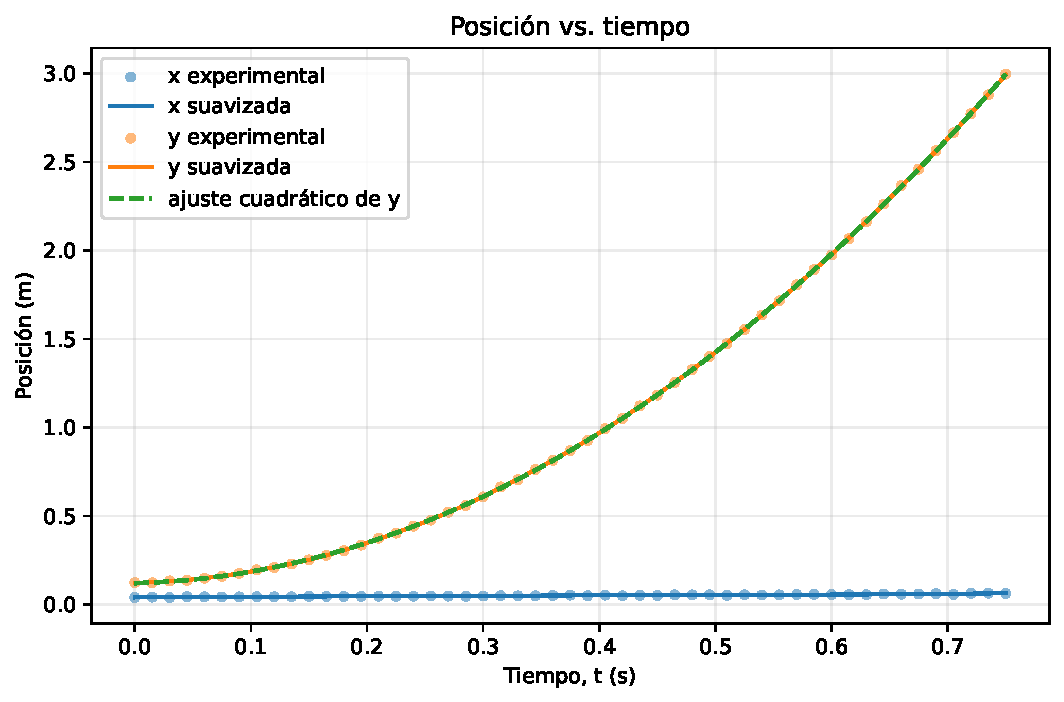
\includegraphics[width=0.95\linewidth]{posicion_tiempo.pdf}
\caption{Coordenadas experimentales, señales suavizadas y ajuste cuadrático de la coordenada vertical.}
\label{fig:position}
\end{figure}
\begin{figure}[H]
\centering
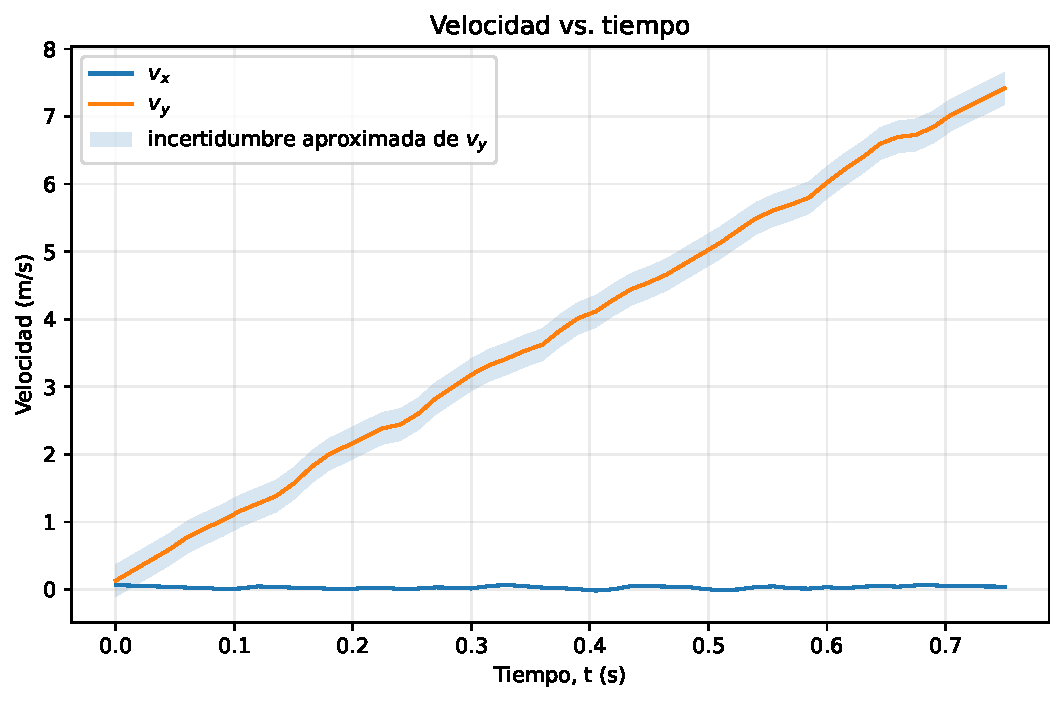
\includegraphics[width=0.95\linewidth]{velocidad_tiempo.pdf}
\caption{Componentes de velocidad obtenidas por derivación numérica.}
\label{fig:velocity}
\end{figure}
\begin{figure}[H]
\centering
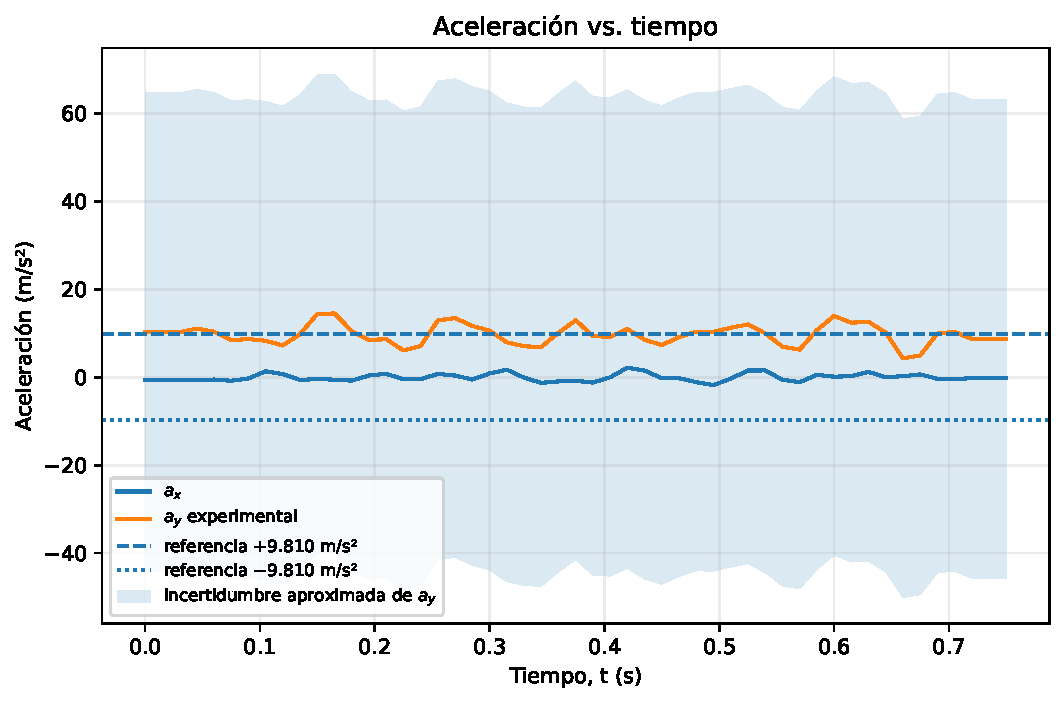
\includegraphics[width=0.95\linewidth]{aceleracion_tiempo.pdf}
\caption{Aceleración numérica y referencias gravitatorias.}
\label{fig:acceleration}
\end{figure}
\begin{figure}[H]
\centering
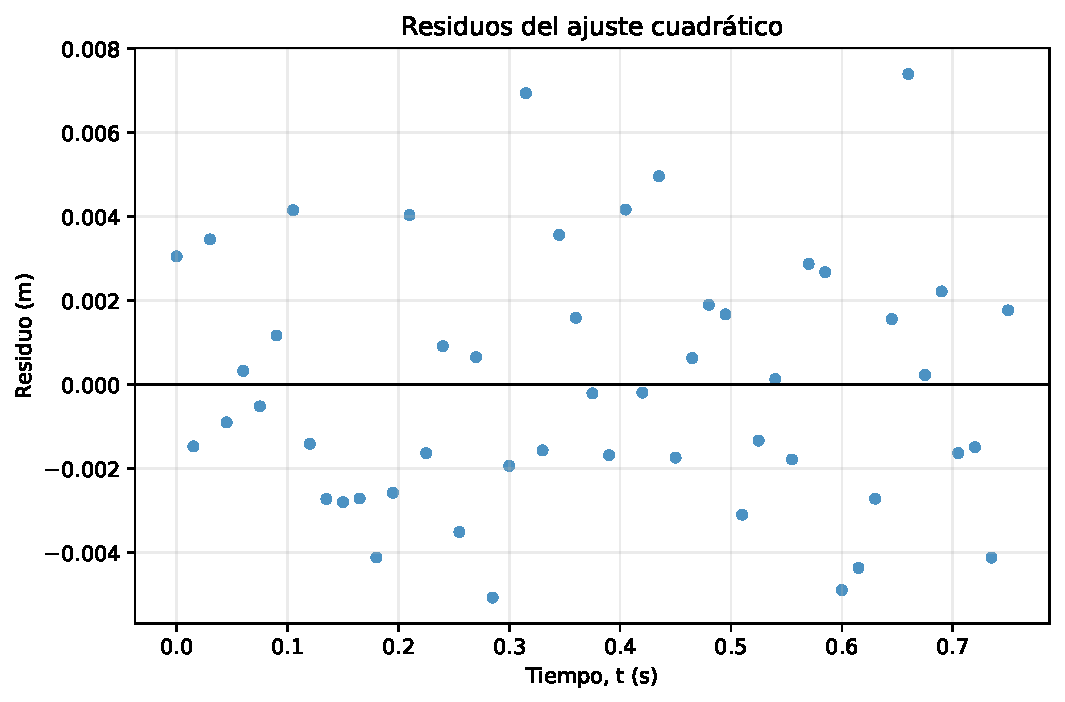
\includegraphics[width=0.95\linewidth]{residuos_ajuste.pdf}
\caption{Residuos del ajuste cuadrático de la posición vertical.}
\label{fig:residuals}
\end{figure}

\section{Discusión}
Se debe valorar si los residuos presentan estructura temporal, tendencia o dispersión creciente. Un patrón sistemático puede indicar perspectiva, escala incorrecta, resistencia del aire, movimiento de la cámara o selección inconsistente del centro del objeto. La incertidumbre de la aceleración del ajuste depende de la dispersión de los datos, del intervalo temporal y de la validez del modelo. La incertidumbre aproximada de las derivadas incluida en las figuras supone errores de posición independientes y muestreo casi uniforme; no sustituye un presupuesto completo de incertidumbre instrumental.

\section{Conclusiones}
El pipeline automatiza la lectura, validación, cálculo cinemático, ajuste de un modelo físico y producción de figuras y tablas. Para una conclusión experimental definitiva se deben reemplazar los datos demostrativos por mediciones propias, documentar calibración y frecuencia de cuadros, y contrastar el ajuste de Python con QtiPlot.

\section*{Disponibilidad y reproducibilidad}
El código fuente, el archivo crudo de demostración y las instrucciones para ejecutar el análisis se distribuyen junto con este informe. Los parámetros de filtrado, la incertidumbre de posición y la gravedad de referencia deben reportarse con cada conjunto experimental.

\bibliographystyle{IEEEtran}
\bibliography{referencias}
\end{document}
